\documentclass[12pt]{article}

\usepackage[utf8]{inputenc}
\usepackage{geometry}
\geometry{a4paper,scale=0.75}
\linespread{1.5}
\usepackage{graphicx} 
\usepackage{float} 
\usepackage{subcaption} 
\usepackage{enumerate}
\usepackage{enumitem}
\usepackage{amsmath}
\usepackage{array}
\usepackage{booktabs}
\usepackage{multirow}
\usepackage{amsfonts}
\usepackage[english]{babel}
\usepackage{amsthm}
\usepackage{dcolumn}
\usepackage{multicol}
\usepackage{stfloats}
\usepackage{lscape}
\usepackage[figuresright]{rotating}
\RequirePackage{pdflscape}
\usepackage[toc,page]{appendix}
\usepackage{geometry}
\usepackage{longtable}
\usepackage{comment}
\usepackage{xcolor}

% -------- enumerated sub-labels (a), (b), … --
\usepackage{enumitem}
\setlist[enumerate,1]{label=(\alph*),ref=\alph*}
% ---------------------------------------------

\usepackage{hyperref}
\hypersetup{hidelinks,
	colorlinks=true,
	allcolors=black,
	pdfstartview=Fit,
	breaklinks=true}
\usepackage{csquotes}
\usepackage{natbib}
\bibliographystyle{apalike}
\newtheorem{definition}{Definition}
\newtheorem{theorem}{Theorem}
\newtheorem{proposition}[theorem]{Proposition}
\newtheorem{lemma}[theorem]{Lemma}
\newtheorem{corollary}[theorem]{Corollary}
\newtheorem*{remark}{Remark}
\newtheorem{example}{Example}
\newtheorem{exercise}{Exercise}
\newtheorem{assumption}{Assumption}[section] % number within sections


\begin{document}

\begin{center}
    ECON 4999B: Quantitative Macroeconomics with AI Integration\\
    {\large \textbf{Tutorial Note: Vector Autoregression (VAR) and Local Projection (LP)}}\\
    Teaching Assistant: Harlly Zhou
\end{center}

The main reference for this tutorial is \textit{Econometrics} by Fumio Hayashi and \textit{Time Series: Theory and Methods} by Peter J. Brockwell and richard A. Davis.

\section{Vector Autoregression (VAR)}
Now we are discussing a vector of time series $\vec{y}_t = (y_{1t}, y_{2t}, \cdots, y_{nt})'$ as an $n \times 1$ vector. Still, \textbf{weak stationarity} is very important. 
\begin{definition}[weak stationarity]
    Consider a time series $\vec{y}_t = (y_{1t}, y_{2t}, \cdots, y_{nt})'$. We say that $\vec{y}_t$ is weakly stationary if:
    \begin{enumerate}
        \item The mean of $\vec{y}_t$ is constant: $\mathbb{E}[\vec{y}_t] = \vec{\mu}$ for all $t$.
        \item The covariance matrix of $\vec{y}_t$ is constant: $\Gamma(j) = \mathbb{E}[(\vec{y}_t - \vec{\mu})(\vec{y}_{t-j} - \vec{\mu})'] = \Sigma$ for all $t$ and $j$.
    \end{enumerate}
\end{definition}
Here are several properties:
\begin{itemize}
    \item $\operatorname{diag}(\Gamma(0)) = \operatorname{diag}(\operatorname{Var}(y_{it}))$;
    \item $\Gamma_{k \ell}(j) = \operatorname{Cov}(y_{kt}, y_{\ell, t-j})$;
    \item $\Gamma(j) = \Gamma(-j)'$ but not $\Gamma(j) = \Gamma(-j)$.
\end{itemize}

Now consider a weakly stationary vector time series $\vec{y}_t$. We can write the $VAR(p)$ model as:
\begin{align*}
    \vec{y}_t = \vec{c} + \Phi_1 \vec{y}_{t-1} + \Phi_2 \vec{y}_{t-2} + \cdots + \Phi_p \vec{y}_{t-p} + \vec{e}_t,
\end{align*}
where $\vec{e}_t\sim WN(0, \Omega)$. Here $\Phi_i$ is an $n \times n$ matrix. We can also write the model in a companion form:
\begin{align*}
    Y_t = FY_{t-1} + E_t,
\end{align*}
where $Y_t$ is an $np \times 1$ vector, $F$ is an $np \times np$ matrix, and $E_t$ is an $np \times 1$ vector such that
\begin{align*}
    Y_t = \begin{bmatrix}
    \vec{y}_t - \vec{\mu}\\
    \vec{y}_{t-1} - \vec{\mu}\\
    \vdots\\
    \vec{y}_{t-p} - \vec{\mu}
    \end{bmatrix},
    F = \begin{bmatrix}
    \Phi_1 & \Phi_2 & \cdots & \Phi_{p-1} &\Phi_p\\
    I_n & 0 & \cdots & 0 & 0\\
    \vdots & \vdots & \ddots & \vdots & \vdots\\
    0 & 0 & \cdots & I_n & 0
    \end{bmatrix},
    E_t = \begin{bmatrix}
    \vec{e}_t\\
    \vec{0}\\
    \vdots\\
    \vec{0}.
    \end{bmatrix}
\end{align*}

For autoregressive models, we need to consider the stability of the model.
\begin{proposition}[stability of VAR model]
    A $VAR(p)$ model is stable if either of the following conditions holds:
    \begin{itemize}
        \item all the roots of $|I_n - \Phi_1 z - \Phi_2 z^2 - \cdots - \Phi_p z^p| = 0$ lie outside the unit circle, where $|\cdot|$ is the modulus of a complex number.
        \item all the eigenvalues of the companion matrix $F$ lie inside the unit circle.
    \end{itemize}
\end{proposition}
The second condition is more used empirically.

Applying the companion form recursively, we get:
\begin{align*}
    Y_t = F^j Y_{t-j} + \sum_{i=0}^{j-1} F^i E_{t-j+i}.
\end{align*}
Then the variances and covariances are given by:
\begin{align*}
    \Gamma(j) &= \operatorname{Cov}(Y_t, Y_{t-j})\\
    &= \operatorname{Cov}(F^j Y_{t-j} + \sum_{i=0}^{j-1} F^i E_{t-j+i}, Y_{t-j})\\
    &= F^j \operatorname{Var}(Y_{t-j})\\
    &= F^j \operatorname{Var}(Y_t),
\end{align*}
where the last equality follows from the fact that $\vec{y}_t$ is weakly stationary. Then how to estimate the variance-covariance matrix? Applying the variance operator on both sides of the companion form, we get:
\begin{align*}
    \Sigma = F \Sigma F' + Q,
\end{align*}
where $Q = \mathbb{E}[E_t E_t']$. We can solve this equation using two methods:
\begin{itemize}
    \item Methods for solving (generalized) Lyapunov equations. A Lyapunov equation is of the form $X = A X A' + C$ and a generalized Lyapunov equation is of the form $B X B' = A X A' + C$.
    \item Recursive method. Plug $\Sigma = \Sigma_0$ into the right hand side and get $\hat{\Sigma}_1 = F \hat{\Sigma}_0 F' + Q$. Choose $\lambda \in (0,1)$ and define $\Sigma_1 = \lambda \hat{\Sigma}_1 + (1-\lambda) \Sigma_0$. Then plug $\Sigma_1$ into the right hand side and get $\hat{\Sigma}_2 = F \hat{\Sigma}_1 F' + Q$. Repeat this process and get $\Sigma_n \to \Sigma$ as $n \to \infty$.
\end{itemize}

To estimate the parameters of the $VAR(p)$ model, we can use the method of maximum likelihood. 

\section{Granger Causality}
Consider a $VAR(p)$ model:
\begin{align*}
    \vec{y}_t = \vec{c} + \Phi_1 \vec{y}_{t-1} + \Phi_2 \vec{y}_{t-2} + \cdots + \Phi_p \vec{y}_{t-p} + \vec{e}_t.
\end{align*}
We would like to test whether the history of $y_{j}$ helps forecast $y_{it}$. This is the concept of \textbf{Granger causality}.
\begin{definition}[Granger causality]
    We say that $y_{jt}$ \textbf{Granger causes} $y_{it}$ if at least one lag of $y_{jt}$ enters the $i$-th equation of the $VAR(p)$ model. That is,
    \begin{align*}
        \big((\Phi_1)_{ij},(\Phi_2)_{ij},\ldots,(\Phi_p)_{ij}\big) \neq (0,0,\ldots,0).
    \end{align*}
    Equivalently, the null hypothesis of no Granger causality from $y_{jt}$ to $y_{it}$ is
    \[
        H_0:(\Phi_1)_{ij}=(\Phi_2)_{ij}=\cdots=(\Phi_p)_{ij}=0.
    \]
\end{definition}

Consider a two-variable $VAR(1)$ model:
\begin{align*}
    \begin{bmatrix}
        y_{1t}\\
        y_{2t}
    \end{bmatrix}
    =
    \begin{bmatrix}
        c_1\\
        c_2
    \end{bmatrix}
    +
    \begin{bmatrix}
        \phi_{11} & \phi_{12}\\
        \phi_{21} & \phi_{22}
    \end{bmatrix}
    \begin{bmatrix}
        y_{1t-1}\\
        y_{2t-1}
    \end{bmatrix}
    +
    \begin{bmatrix}
        \epsilon_{1t}\\
        \epsilon_{2t}
    \end{bmatrix}
\end{align*}
If $\phi_{12} \neq 0$, then $y_2$ Granger causes $y_1$. If $\phi_{12} = 0$, then $y_2$ does not Granger cause $y_1$.

\subsection{Forward-Looking Variables}
Consider the asset pricing equation:
\begin{align*}
    P_t = \mathbb{E}_t \sum_{s=1}^{+\infty} (1+r)^{-s} D_{t+s}.
\end{align*}
We say that $P_t$ is a \textbf{forward-looking} variable if it is a function of future variables. 

Suppose that $D_t = u_t + \delta u_{t-1} + \nu_t$. Then$\mathbb{E}_t D_{t+s} = \delta u_t$ if $s=1$, or zero, otherwise. Then $P_t = \frac{\delta u_t}{1+r}$. In $VAR(1)$ form, we have
\begin{align*}
    \begin{bmatrix}
        P_{t}\\
        D_{t}
    \end{bmatrix}
    =
    \begin{bmatrix}
        0 & 0\\
        1+r & 0
    \end{bmatrix}
    \begin{bmatrix}
        P_{t-1}\\
        D_{t-1}
    \end{bmatrix}
    +
    \begin{bmatrix}
        \frac{\delta u_t}{1+r}\\
        u_t + \nu_t
    \end{bmatrix}.
\end{align*}
This specification shows that $P_t$ Granger causes dividend $D_t$. In general, forward-looking variables (consumption, asset prices, \textit{etc.}) Granger cause real variables.

\section{Structural VAR}
\subsection{What is a Structural Model?}
We can always observe macroeconomic variables. Using the AIC/BIC, we can pin down the order $p$ and then make an estimation. Although the residuals are white noises, $e_{it}$ and $e_{jt}$ are not independent. Consider a vector of variables, GDP growth, inflation, and federal funds rate. If the residuals are independent, then we can understand them as the structural shock to productivity, inflation, and monetary policy. However, the residuals are correlated with each other, which can be easily seen from an IS-LM model. To generate the purified shocks, we need a structural model.

With an established theory, it is not always easy to separate the contemporaneous observation. A general structural model is of the form:
\begin{align*}
    A_0 \vec{y}_t = A_1 \vec{y}_{t-1} + A_2 \vec{y}_{t-2} + \cdots + A_p \vec{y}_{t-p} + R \vec{\nu}_t,
\end{align*}
where $\mathbb{E}[\vec{\nu}_t \vec{\nu}'_s] = \Sigma$, a diagonal matrix, if $t=s$ and zero, otherwise. This $\vec{\nu}_t$ is the \textbf{structural shock}. How does structural model interact with reduced-form model? The reduced-form model is of the form:
\begin{align*}
    \vec{y}_t &= A_0^{-1} A_1 \vec{y}_{t-1} + A_0^{-1} A_2 \vec{y}_{t-2} + \cdots + A_0^{-1} A_p \vec{y}_{t-p} + A_0^{-1}R \vec{\nu}_t\\
    &:= \Phi_1 \vec{y}_{t-1} + \Phi_2 \vec{y}_{t-2} + \cdots + \Phi_p \vec{y}_{t-p} + \vec{e}_t,
\end{align*}
where $\mathbb{E}[\vec{e}_t \vec{e}'_s] = \Omega$ (not necessarily a diagonal matrix) if $t=s$ and zero, otherwise. To recover $\vec{\nu}_t$ from $\vec{e}_t$, we have
\begin{align*}
    \Phi_i = A_0^{-1} A_i, \qquad \Omega = A_0^{-1} R \Sigma R' (A_0^{-1})'.
\end{align*}

Whatever model we use, the ultimate goal is to estimate how a variable responds to a structural shock. As time passes, the response also decays. This response as a function of time is called the \textbf{impulse response function} (IRF).

\subsection{Impulse Response Function (IRF)}
A $VAR(p)$ model can be written as
\[
    \vec{y}_t = \vec{\mu} + \Psi(L) \vec{e}_t.
\]
Suppose that $\vec{e}_t = P \vec{\nu}_t$ for some structural shock $\vec{\nu}_t$. Then
\begin{align*}
    \frac{\partial y_{i, t+s}}{\partial \nu_{jt}} = [\Psi_s P]_{ij}.
\end{align*}

Consider the vector
\[
    \vec{y}_t =
    \begin{bmatrix}
        \Delta \log(\text{GDP}_t)\\
        \Delta \log(\text{CPI}_t)\\
        FFR_t
    \end{bmatrix}.
\]
The GDP and CPI variables are log differences, while the federal funds rate is kept in levels. Using quarterly data from FRED, AIC selects a $VAR(3)$. We can then empirically ``invert'' the model and get the impulse response function:
\begin{figure}[H]
    \centering
    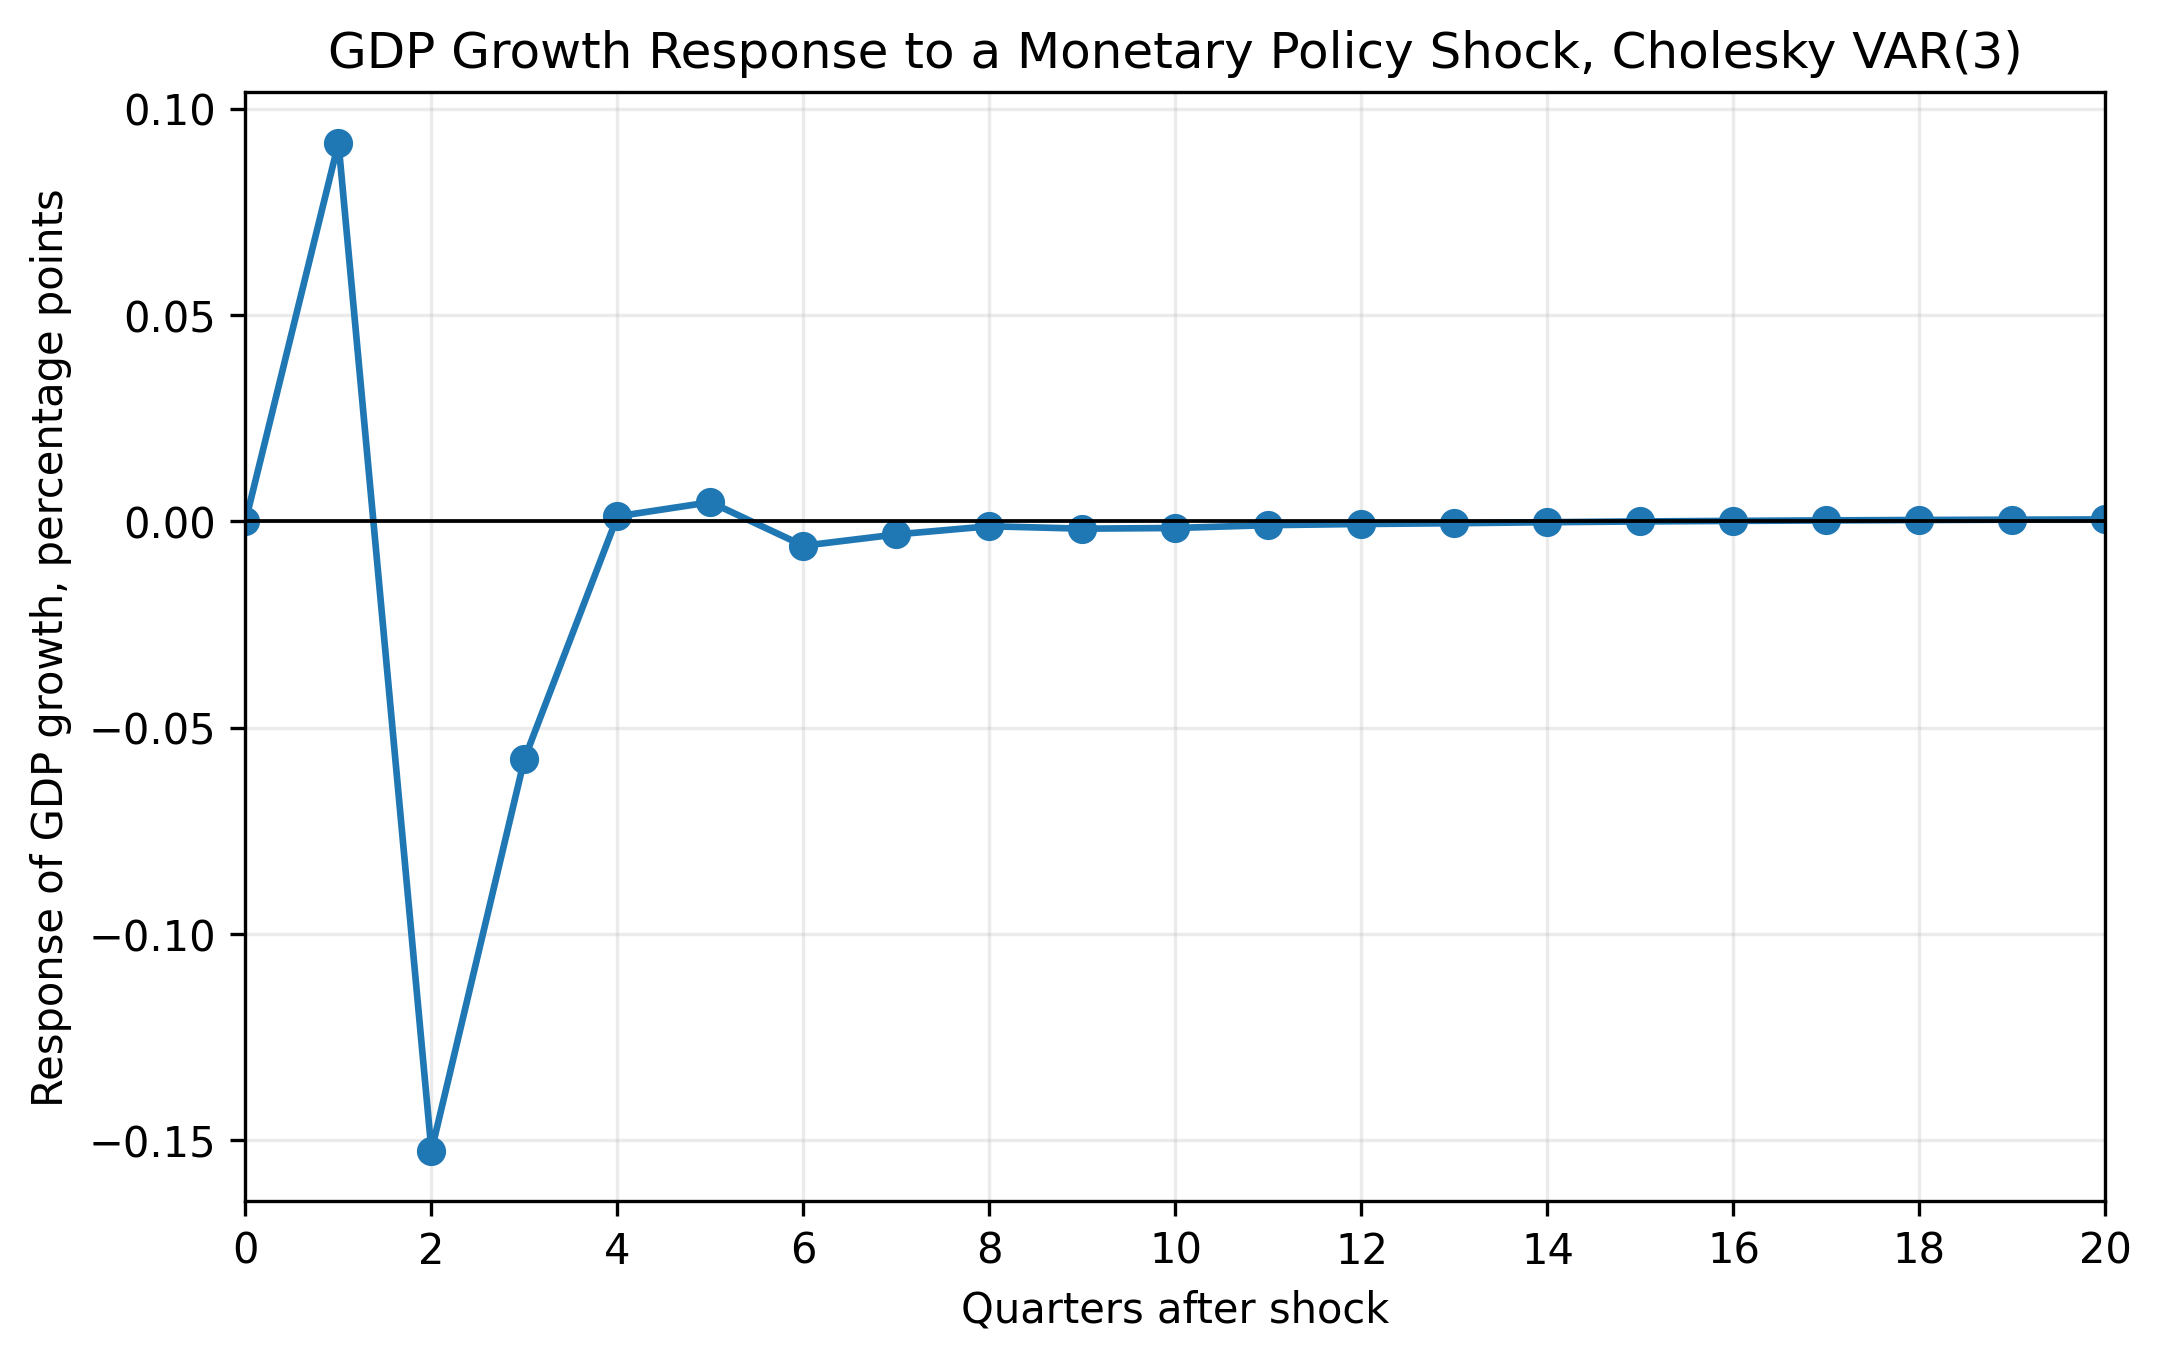
\includegraphics[width=0.8\textwidth]{irf_gdp_growth_to_mp_cholesky.png}
    \caption{Impulse response of GDP growth to a Cholesky monetary policy shock.}
    \label{fig:irf-gdp-growth-mp}
\end{figure}
Figure \ref{fig:irf-gdp-growth-mp} shows the response of GDP growth to a one-standard-deviation monetary policy shock, which raises the federal funds rate by about $0.71$ percentage points on impact. The contemporaneous GDP response is zero by construction under the Cholesky ordering, and the response becomes negative over the following quarters.

Although we get the impulse response, we do not know whether the response is statistically significant. There are two methods to empirically test this:
\begin{itemize}
    \item Monte Carlo simulation: simulate the parameters using the asymptotic distribution of the parameters of the model.
    \item Bootstrap: simulate the data based on the estimated model and use the simulated data to estimate the model again.
\end{itemize}
Using the two methods, we can construct confidence bands for the impulse response function. If the confidence bands do not overlap with zero, then the response is statistically significant.
\begin{figure}[H]
    \centering
    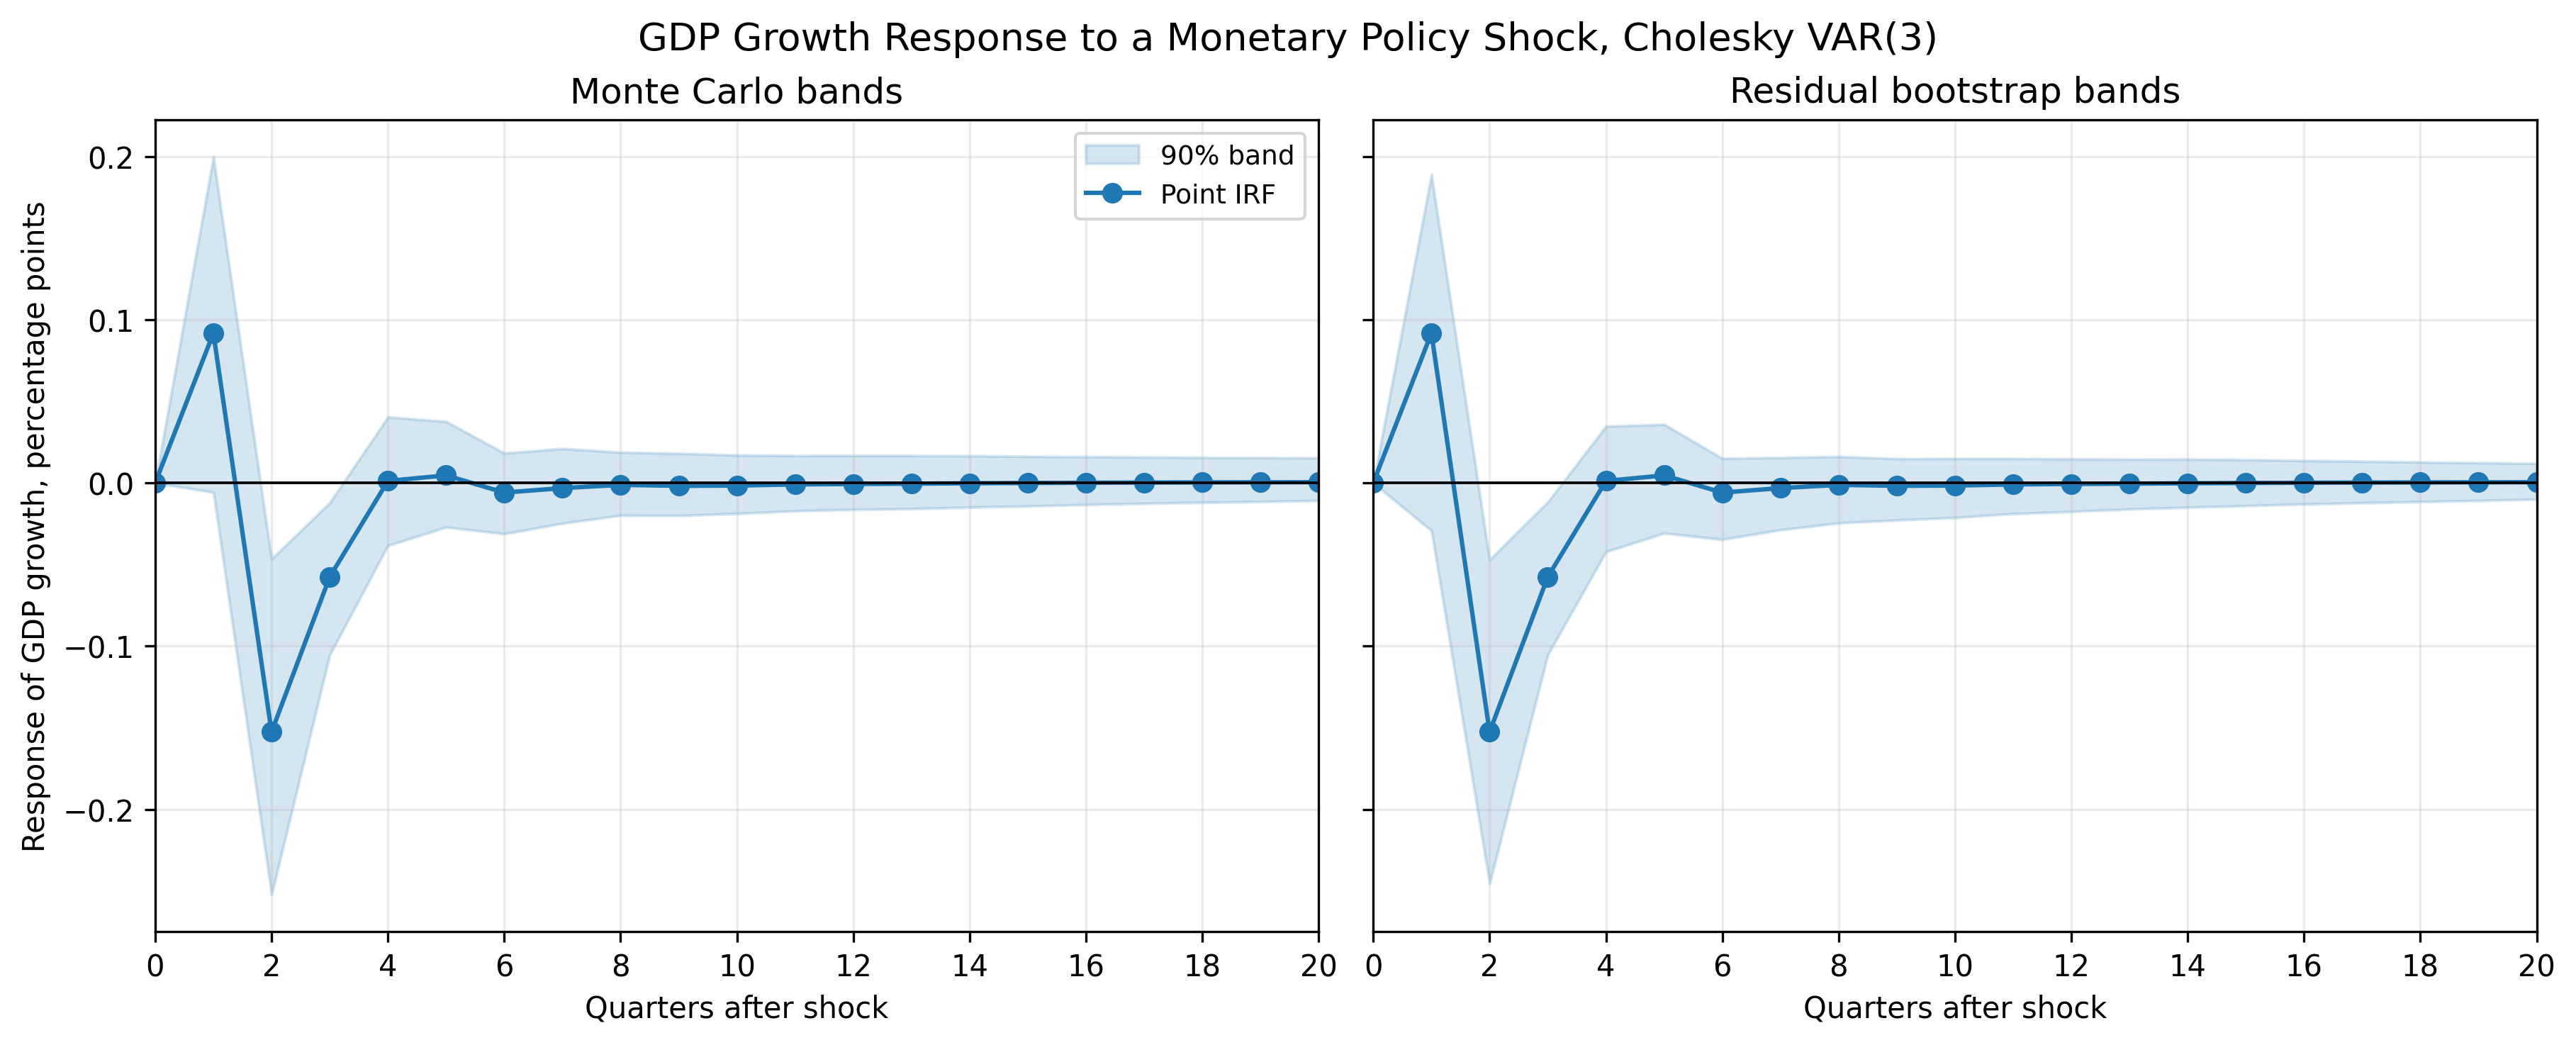
\includegraphics[width=0.95\textwidth]{irf_gdp_growth_to_mp_mc_bootstrap.png}
    \caption{Impulse response of GDP growth to a Cholesky monetary policy shock with Monte Carlo and bootstrap bands.}
    \label{fig:irf-gdp-growth-mp-mc-bootstrap}
\end{figure}
Figure \ref{fig:irf-gdp-growth-mp-mc-bootstrap} reports the same GDP-growth response with pointwise $90\%$ uncertainty bands. The left panel draws VAR coefficients from their asymptotic distribution, while the right panel uses residual bootstrap samples generated from the estimated $VAR(3)$ model.

\subsection{Estimation and Identification}
Recall that to recover the structural shocks from a reduced-form model, we need the following parameters:
\begin{align*}
    \Phi_i = A_0^{-1} A_i, \qquad \Omega = A_0^{-1} R \Sigma R' (A_0^{-1})',
\end{align*}
where $\{\Phi_i\}$ provides $p \times n^2$ parameters and $\Omega$ provides $n(n+1)/2$ parameters. On the other hand, we need to identify $\Sigma$, which has only the $n$ entris on its diagonal, $R$ with $n^2$ entries, and $\{A_i\}$ with $(p+1) \times n^2$ parameters. As a result, we require $n/2 + 3n^2/2 > 0$ restrictions to identify the model. 

A natural restriction is to set $\operatorname{diag}(A_0) = I_n$ so that each equation $i$ can have $y_{it}$ on the LHS. There is still $3n^2/2 - n/2$ restrictions needed. Note that the variance-covariance matrix $\Omega$ is related to $\Sigma$ in a \textit{sandwich form}, that is, $\Omega = B \Sigma B'$. This rings the bell for a decomposition method.
\begin{lemma}[LDL decomposition]
    For any variance-covariance matrix $\Omega$, there exists a lower triangular matrix $\mathcal{L}$ and a diagonal matrix $\Delta$ such that 
    \begin{itemize}
        \item $\operatorname{diag}(\mathcal{L}) = I$, and
        \item $\Omega = \mathcal{L} \Delta \mathcal{L}'$.
    \end{itemize}
\end{lemma}
Then we can let $R = I_n$ and $A_0 = \mathcal{L}^{-1}$ so that there is in total $n^2 + n(n-1)/2$ restrictions, which is just enough for identification. As a result, $\vec{\nu}\sim \mathcal{N}(0, \Delta)$.

This LDL method is good in since the assumption for $R$ and $A_0$ are very clear. However, the structural shock is not of unit variance. To retain this property, we can use the \textbf{Cholesky decomposition} instead, where $R = \Delta ^{1/2}$ and $A_0 = \mathcal{L}^{-1}$. In this way, we naturally have $\vec{\nu}_t \sim \mathcal{N}(0, I_n)$.

\begin{example}[monetary policy shock]
We now try to identify the monetary policy shock we used in the IRF example. The vector is ordered as
\[
    \vec{y}_t =
    \begin{bmatrix}
        \Delta \log(\text{GDP}_t)\\
        \Delta \log(\text{CPI}_t)\\
        FFR_t
    \end{bmatrix}.
\]
The ordering means that output growth is ordered first, inflation second, and the federal funds rate last. Under Cholesky identification, the monetary policy shock is therefore the third structural shock.

\textbf{Step 1: Choose the lag length.} AIC selects $p=3$.

\textbf{Step 2: Estimate the reduced-form VAR.} With $p=3$, the estimated reduced-form coefficients are reported in Table \ref{tab:var-regression-result}.

\begin{table}[H]
    \centering
    \caption{Reduced-form $VAR(3)$ coefficient estimates}
    \label{tab:var-regression-result}
    \begin{tabular}{lccc}
        \toprule
        Regressor & GDP growth & Inflation & FFR \\
        \midrule
        Constant & 0.797 & 0.136 & -0.203 \\
        GDP growth$_{t-1}$ & 0.027 & -0.015 & 0.170 \\
        Inflation$_{t-1}$ & -0.183 & 0.480 & -0.107 \\
        FFR$_{t-1}$ & 0.129 & 0.145 & 1.195 \\
        GDP growth$_{t-2}$ & 0.104 & 0.000 & 0.093 \\
        Inflation$_{t-2}$ & -0.037 & 0.048 & 0.383 \\
        FFR$_{t-2}$ & -0.344 & -0.118 & -0.474 \\
        GDP growth$_{t-3}$ & 0.032 & 0.017 & 0.072 \\
        Inflation$_{t-3}$ & -0.054 & 0.239 & 0.066 \\
        FFR$_{t-3}$ & 0.228 & -0.011 & 0.206 \\
        \bottomrule
    \end{tabular}
\end{table}

\textbf{Step 3: Apply LDL and Cholesky identification.} From the residuals, the estimated variance-covariance matrix is
\[
    \widehat{\Omega} =
    \begin{bmatrix}
        1.0489 & 0.1040 & 0.2062 \\
        0.1040 & 0.1987 & 0.0815 \\
        0.2062 & 0.0815 & 0.5516
    \end{bmatrix}.
\]
Its LDL decomposition is
\[
    \widehat{\Omega}
    =
    \mathcal{L}\Delta \mathcal{L}',
    \qquad
    \mathcal{L}
    =
    \begin{bmatrix}
        1.0000 & 0 & 0 \\
        0.0991 & 1.0000 & 0 \\
        0.1966 & 0.3239 & 1.0000
    \end{bmatrix},
    \qquad
    \Delta
    =
    \begin{bmatrix}
        1.0489 & 0 & 0 \\
        0 & 0.1884 & 0 \\
        0 & 0 & 0.4913
    \end{bmatrix}.
\]
To normalize the structural shocks to have unit variance, define the Cholesky impact matrix
\[
    P = \mathcal{L}\Delta^{1/2}
    =
    \begin{bmatrix}
        1.0241 & 0 & 0 \\
        0.1015 & 0.4341 & 0 \\
        0.2014 & 0.1406 & 0.7009
    \end{bmatrix}.
\]
Then the reduced-form residuals satisfy $\hat{e}_t=P\hat{\nu}_t$, so the recovered structural shocks are
\[
    \hat{\nu}_t = P^{-1}\hat{e}_t.
\]
The monetary policy shock is the third element of $\hat{\nu}_t$.

\textbf{Step 4: Recover the monetary policy shock.} Figure \ref{fig:mp-shock-distribution} plots the recovered monetary policy shock. Because of the Cholesky normalization, the shock has approximately mean zero and unit variance.

\begin{figure}[H]
    \centering
    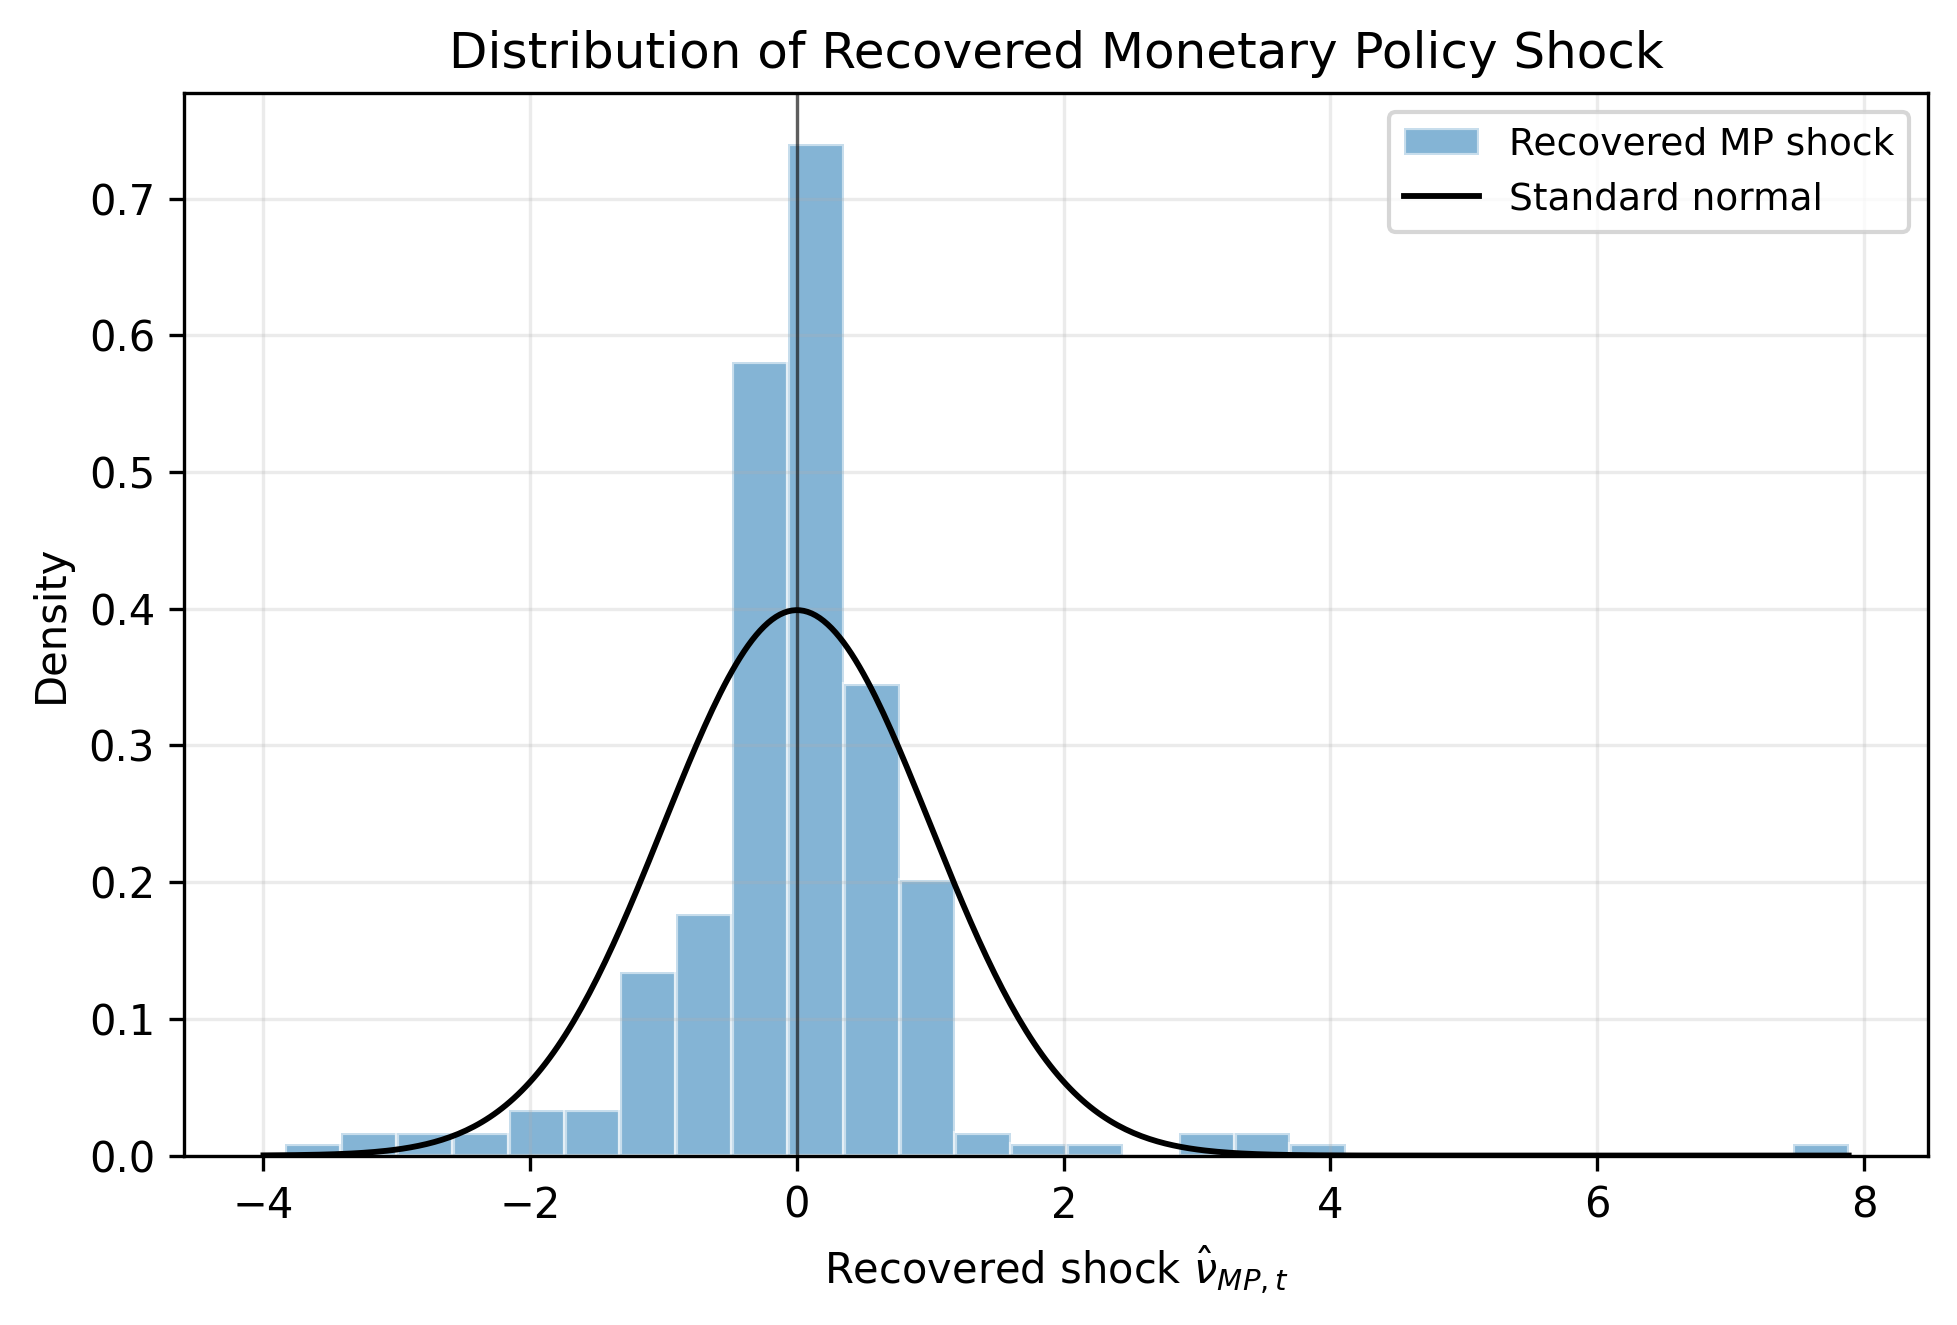
\includegraphics[width=0.75\textwidth]{mp_shock_cholesky_distribution.png}
    \caption{Distribution of the recovered monetary policy shock using Cholesky identification.}
    \label{fig:mp-shock-distribution}
\end{figure}
\end{example}

\subsection{VAR Estimation in Literature}
The most typical use of VAR in the literature is to purify the monetary policy shock, and a representative paper is Bernanke and Mihov (QJE, 1998). The ultimate goal is to show how a monetary policy shock affects the economy. The structural model is of the form:
\begin{align*}
    Y_t &= B_0 Y_t + f(Y_{t-1}, P_{t-1}, \cdots) + R \nu^Y_t,\\
    P_t &= G_0 P_t + D_0 Y_t + g(Y_{t-1}, P_{t-1}, \cdots) + S \nu^P_t,
\end{align*}
where $Y = [GDP, PDGP, PCM]'$ (GDP, GDP deflator, commodity prices) are non-policy variables and $P = [FF, TR, NBR]'$ (federal funds rate, total bank reserves, non-borrowed reserves) are policy variables. The VAR residuals (innovations) are
\begin{align*}
    \mu^Y_t &= (I - B_0)^{-1} R \nu^Y_t,\\
    \mu^P_t &= (I - G_0)^{-1} D_0 (1-B_0)^{-1} R \nu^Y_t + (I - G_0)^{-1} S \nu^P_t.
\end{align*}
The orthogonal component in $\mu^P$ w.r.t. $\mu^Y$ is $e_t : = (I - G_0)^{-1} S \nu^P_t$. Now we can use the vector $\mu^Y$, $\mu^P$ to recover $\nu^P$.

By intuition, the bank reserve market has the following relations:
\begin{align*}
    e_{TR} &= -\alpha e_{FF} + v^d,\\
    e_{BR} &= \beta (e_{TR} - e_{DISC}) + v^b,\\
    e_{NBR} &= \phi^d v^d + \phi^b v^b + v^s.
\end{align*}
Together with the market clearing condition $e_{TR} = e_{BR} + e_{NBR}$, and an additional assumption $e_{DISC} = 0$, we have
\begin{align*}
    \begin{bmatrix}
        (\alpha + \beta) & 0 & 0\\
        \alpha & 1 & 0\\
        0 & 0 & 1
    \end{bmatrix}
    \begin{bmatrix}
        e_{FF}\\
        e_{TR}\\
        e_{NBR}
    \end{bmatrix}
    =
    \begin{bmatrix}
        -(\phi^b+1) & 1-\phi^d & -1\\
        0 & 1 & 0\\
        \phi^b & \phi^d & 1
    \end{bmatrix}
    \begin{bmatrix}
        v^b\\
        v^d\\
        v^s
    \end{bmatrix}.
\end{align*}
We can empirically get $e_{FF}, e_{TR}, e_{NBR}$ from the residuals. Now we get the ``$\Omega$'' matrix: the variances and covariances of the residuals, which, in total, have 6 pieces of information. On the other hand, however, we need to estimate 7 things: $\alpha, \beta, \phi^d, \phi^b$ and the variances of the structural shocks. We need one more restriction to identify the model.

Now you need the intuition. The assumption the paper made is $\alpha = 0$, that is, the total reserve is inelastic to the federal funds rate. This is reasonable because the total reserve is always subject to many operational regulations, which is kind of inelastic. Then everything else is identified, and we can plot the IRF of the non-policy variables to a pure monetary policy shock $v^s$.

\section{Local Projection}
VAR is good to find the structural shocks. However, in the previous example, we saw that there is a very artificial assumption $\alpha = 0$. No matter how intuition this seems, it is less scientific. Therefore, \underline{after the structural shock is identified}, we can use the \textbf{local projection method} to estimate the impulse response function.

Recall that IRF is the response of a variable to a structural shock after $h$ periods. Then we can estimate the IRF by regressing the variable (univariate) on the structural shock and its lags, with controls:
\begin{align*}
    y_{t+h} = c + \sum_{q=1}^Q \phi_q^{(h)} y_{t-q} + \sum_{m=0}^M \beta_m^{(h)} x_{t-m} + \sum_{r=1}^R \vec{\gamma}_r^{(h)} \vec{W}'_{t-r} + u_{t+h|t},
\end{align*}
where $y$ is the variable of interest, $x$ is the structural shock, and $\vec{W}$ is a vector of controls. The impulse responses of $x_t$ on future values of $y$ are
\begin{align*}
    IRF = \{\beta_0^{(0)}, \beta_0^{(1)}, \ldots, \beta_0^{(H)}\}.
\end{align*}
You can also use Monte Carlo or Bootstrap to construct confidence bands for the IRF.

\begin{figure}[H]
    \centering
    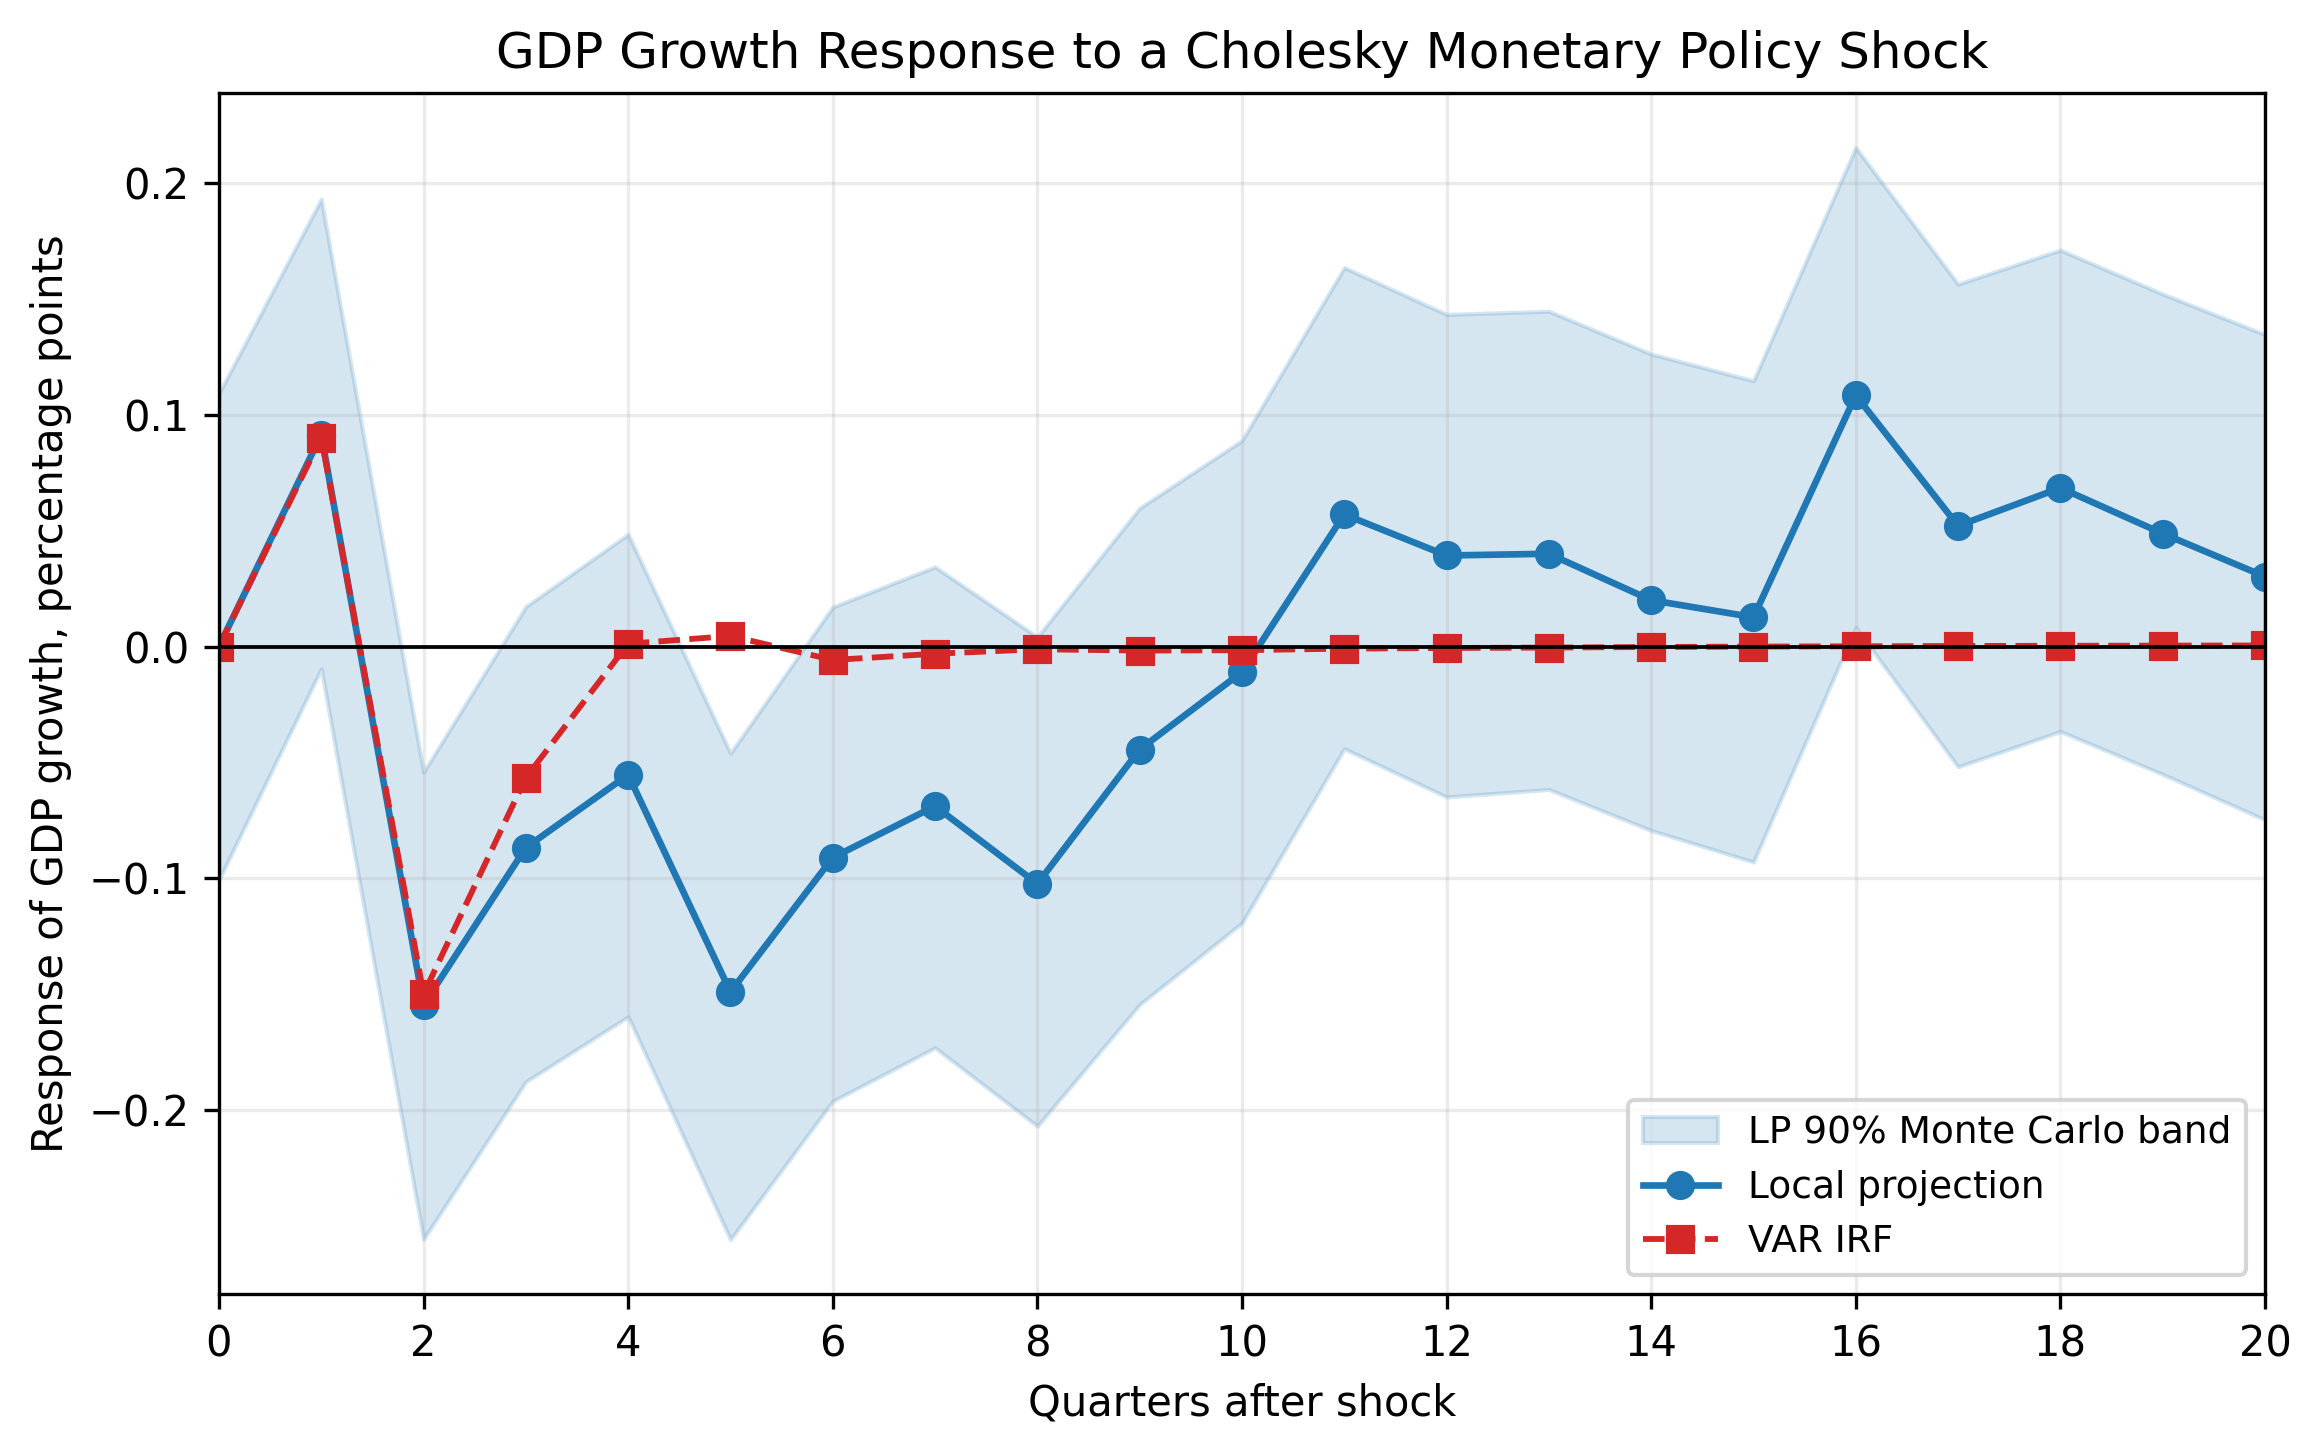
\includegraphics[width=0.85\textwidth]{lp_vs_var_irf_gdp_mp.png}
    \caption{GDP growth response to the Cholesky monetary policy shock: local projection and VAR.}
    \label{fig:lp-var-gdp-mp}
\end{figure}

Figure \ref{fig:lp-var-gdp-mp} uses the Cholesky monetary policy shock recovered above as $x_t$. The local projection regression controls for three lags of GDP growth, inflation, and the federal funds rate. The blue shaded area is a pointwise $90\%$ Monte Carlo confidence band for the local projection estimate. The dashed red line is the VAR impulse response computed from the same Cholesky identification; no confidence band is shown for the VAR response in this figure.

\end{document}